%!TEX root = ../report.tex
\documentclass[../report.tex]{subfiles}

\begin{document}
    \section{Methodology}
    \label{sec:methodology}
    This section details the methodological approach employed to evaluate the efficacy of semantic segmentation models trained on synthetic data generated using Unreal Engine with the AirSim plugin. 
    We propose 2 staged approaches consisting of 1. Synthetic Data Generation 2. Training and Evaluation of Semantic Segmentation. 
    
    \subsection{Synthetic Data Generation}
    \subsubsection{AirSim Setup}
    To generate the synthetic data, set up Unreal Engine Project (UE versions 4.27+) with AirSim plugin integration using the Colosseum repository \cite{colosseumgithub} and follow the documentation \cite{airsimdoc} which exposes APIs to interact with the vehicle in the simulation programmatically using a simulated quadrotor, simulated car or computer vision mode.
    AirSim provides a configuration for users to customize the camera settings to capture the data such as CaptureSettings with ImageType, Width, Height, and FOV\_Degrees, etc. which is a key feature for diverse data generation. 
    In order to balance computational demands and preserve visual fidelity, a resolution of 1280x720 (720p) standard High Definition (HD) is used. We selected 3 to 4 environments to generate the datasets for our semantic segmentation evaluation with City Park (UE 5.2.1), Downtown West (UE 5.2.1), neighborhood (4.27.2), and Landscape Mountain's Village environment (4.27.2). 
    To achieve optimal segmentation annotations, carefully configured material properties in Unreal Engine (UE) using opaque blend modes and default Lit shading models. To eliminate potential rendering artifacts, we have eliminated post-process volumes from the UE environment.
    
    \subsubsection{Waypoint Collector}
    To reproduce the data collection process, a graphical user interface utilizing PyQt5 is developed to facilitate efficient waypoint collection with real-time camera position and orientation representation as shown in figure~\ref{fig:waypoint_collector}. Before generating the data, run the UE simulation from the player's start position to store the camera coordinates (X, Y, Z) and orientation (W, X, Y, Z) in a JSON format using AirSim's simGetVehiclePose API.
    This system captures camera positions at predefined intervals, maintaining a minimum distance of 0.5 meters between each waypoint to ensure comprehensive and diverse scene coverage. This approach ensures both precision and efficiency in our waypoint collection process which can be used for multi-altitudes.
    
    \begin{figure}[ht]
        \centering
        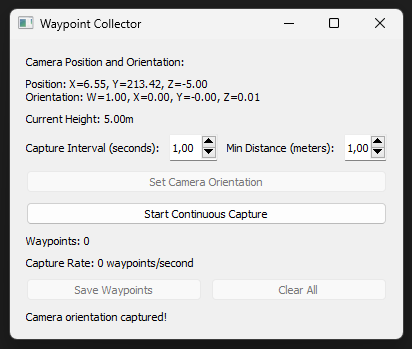
\includegraphics[width=0.9\linewidth]{figures/waypoint_collector.png}
        \caption{Waypoint Collector: a default interval and minimum distance is set with camera's orientation to collect waypoints from UE environment.}
        \label{fig:waypoint_collector}
    \end{figure}
    
     \subsubsection{Segmentation Data Generation}
     Our implementation showcases strategies for semantic labeling of desired objects to assign segmentation that effectively addresses the unique challenges posed by different Unreal Engine versions, particularly concerning AirSim integration limitations. In environments built with Unreal Engine 4.27.2, we developed a label-based mapping approach, primarily due to inconsistencies in how AirSim's simListSceneObjects API capturing the scene objects by missing some of the actors. This challenge notably impacted InstancedFoliageActors, such as trees and vegetation. To overcome this, we created a label mapping JSON that maps all the scene objects to their corresponding semantic classes using precise regex patterns. This mapping is integral to our data generation tool, which adeptly assigns appropriate segmentation IDs to every object in the scene. In contrast, for Unreal Engine 5.2.1 environments, we adopted an efficient tag-based system. Here, objects are tagged with predefined classes like building, road, tree, vehicle, and human, etc. We then extract all tagged objects using a custom object extractor executed within the UE environment's python developer tool. Using these tagged objects segmentation IDs are assigned utilizing AirSim's simSetSegmentationObjectID API. Both approaches adhere to a unified segmentation color scheme of RGB format \cite{airsimsegrgbtxt}, with buildings (196, 30, 8), roads (102, 16, 239), trees (11, 236, 9), vegetation (153, 108, 6), vehicles (242, 107, 146), humans (255, 255, 255), and clutter (0, 0, 0). Prior to assigning new segmentation IDs, our system rigorously resets all existing IDs to 0, ensuring pristine segmentation masks. This dual methodology not only guarantees consistent semantic labeling across various Unreal Engine versions but also enriches the quality and reliability of the generated segmentation masks. 

     \begin{figure}[ht]
        \centering
        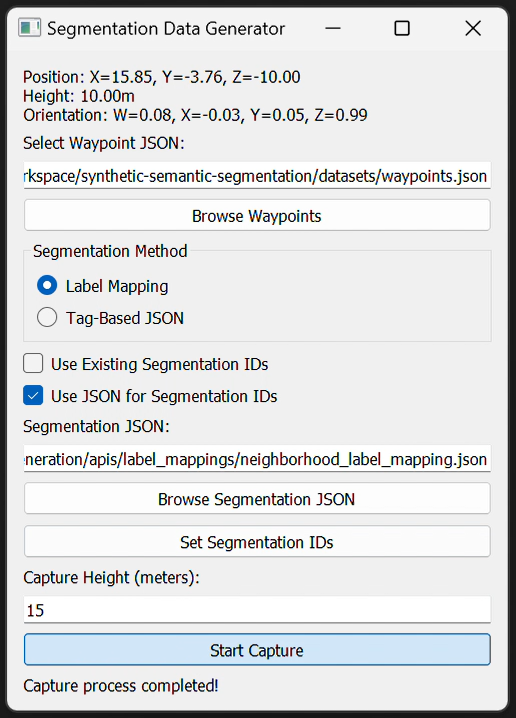
\includegraphics[width=0.9\linewidth]{figures/segmentation_data_generator.png}
        \caption{Data generation for semantic segmentation tasks: a tool which uses the waypoints with multi-altitudes based on user's preferences.}
        \label{fig:segmentation_data_generator}
    \end{figure}
    
     Figure~\ref{fig:segmentation_data_generator} represents the data collection using the Waypoints generated from the waypoint collector tool by specifying the required capture height with the North-East-Down (NED) coordinate system, which utilizes camera height as a negative Z-coordinate. The collected data are categorized and stored in height-specific directories, such as "10m", "15m", or "25m". In addition, the system logs the comprehensive metadata for each collection, which includes capture parameters, ensuring robust data provenance. This approach guarantees consistent and reproducible data collection across various altitudes, crucial for analyzing the impact of height on segmentation performance and developing effective segmentation models at different flying heights.

    In our approach, the time analysis for data generation reveals that capturing each waypoint typically takes around 1 second. Once a waypoint is established, the subsequent data generation process involves camera positioning, capturing RGB images, generating segmentation masks, verifying the data, and storing it averages about 3 seconds per image pair. From one of our data collection sequences, the results revealed that the capture of 34 image pairs was achieved in 99.58 seconds with no quality issues or failed captures. Based on this performance, we can anticipate that generating a dataset of 1000 image pairs would require approximately less than an hour (50 minutes) dedicated solely to the data generation phase.
    This timeline ensures an efficient workflow while maintaining the quality and accuracy of our data collection and generation processes. 

    \subsection{Training and Evaluation Framework}
    The training strategies are followed from the paper \begin{quote} "UAVid: A Semantic Segmentation Dataset for UAV Imagery" \cite{lyu2020uavid}.
    \end{quote} The generated synthetic data set is systematically organized into train, validation, and test splits, adhering to the author's strategic ratio of 3:1:2. Each split comprises paired RGB images alongside their corresponding segmentation masks, captured at desired altitudes. Datasets collected from multiple environments are combined to train and evaluate against the real dataset. 

    \subsubsection{Model Architecture and Training}
    Our framework employs two semantic segmentation architectures: UNet with a ResNet34 backbone, an encoder-decoder architecture, and a transformer architecture, SegFormer-B3, both recognized for their exceptional performance in segmentation tasks. The implementation of UNet is facilitated by the established segmentation models library from PyTorch \cite{unetsmpmodel}, while the SegFormer model is integrated using the HuggingFace model \cite{huggingfacesegformermodel}. 
    Both architectures are standardized through resizing and normalization using mean(0.485, 0.456, 0.406) and standard deviation(0.229, 0.224, 0.225) to match the ImageNet pre-training statistics. We apply data augmentation for train split, such as left-to-right flip randomly, color augmentation, including random hue operation, random contrast operation, random brightness operation, and random saturation operation.
    For real-world datasets, an additional color mapping mechanism ensures consistency between synthetic and real data by converting real-world mask colors to match the synthetic labels for visualization of predictions during evaluation.

    We optimize our model using an exponential learning rate decay schedule, beginning at $10^{-4}$ and decreasing to $10^{-7}$. When using pretrained models, setting the encoder at $10^{-5}$ to preserve its features while allowing the decoder to adapt more rapidly as per the paper \cite{lyu2020uavid}.
    Key training hyperparameters includes, batch size: 32, training epochs: 35, Weight decay: $10^{-4}$, input resolution: 512×512 pixels, and early stopping patience: 5 epochs. To mitigate overfitting and enhance efficiency, we implement early stopping based on validation mean Intersection over Union (mIoU). If no improvement is noted over 5 epochs, training ceases, retaining the best model weights. 

    For performance analysis, we track metrics: Mean Intersection over Union (mIoU), Per-class IoU scores, Training and Validation loss. 
    All experiments are logged using Weights \& Biases (wandb), providing detailed information on training progress and ensuring the reproducibility of the results in various experimental setups.
    We have outlined several hypotheses to explore using both synthetic and real dataset experiments with the specified semantic segmentation models and configurations.   
    
\end{document}
